Our next algorithmic primitive involves \emph{unstructured
  search}. The basic idea is that we have a database $\mathcal{D}$ of
$d$ entries $x_i \in \mathcal{D}$, and
a single marked item $x_m$ we are searching for inside that
database. ``Unstructured'' means that there is no binary search tree,
categories, or other internal scaffolding that a search could use; we
can only check an entry against an oracle function $f: \mathcal{D} \to
\{0, 1\}$ that returns $1$ if $i=m$ and otherwise returns $0$,
i.e. $f(x_i) = \delta_{im}$.
This is analogous to trying entries in a combination lock until the
lock opens.

With a quantum computer, we can promote the database to an algebra
$\mathcal{A}_\mathcal{D}$, with a projector $\Pi_m=\Pi_m^{(Z)}$ onto the marked
item; this answers ``yes'' or ``no'' when presented with a state
$\pi^{(Z)}_i$ representing item $x_i$, and thus encodes $f$:
\[
  \pi^{(Z)}_i(\Pi_m) = \delta_{im} = f(x_i).
\]
In \texttt{yaw}, this takes the form:
  \begin{minted}
     [
frame=lines,
framesep=2mm,
baselinestretch=1.2,
bgcolor=AliceBlue,
fontsize=\footnotesize,
linenos
]{slurm}
    *> def f(i):
    ...    proj(Z, i) | char(Z, m)
\end{minted}
Quantumly, our best bet is to try everything at
once. This is most naturally represented by the state $\pi_+ = \pi^{(X)}_0$,
which has a corresponding dual projector $\Pi_+=\Pi_0^{(X)}$.
We will focus on the subalgebra $\mathcal{A}_{\Pi} = \langle \Pi_m, \Pi_+\rangle \subseteq \mathcal{A}_d$ generated by the
secret answer $\Pi_m$ and the parallel guess $\Pi_+$, since these are
the two distinguished operators we have at hand.
The goal will be to construct an operator that maps the initial guess
$\pi_+$ to the correct answer $\pi_m = \pi^{(Z)}_m$.
A simple ansatz is time evolution by some Hamiltonian $H$
contained in the subalgebra:
\[
  e^{-iHt} \triangleleft \pi_+ \overset{?}{=} \pi_m, \quad H \in \mathcal{A}_{\Pi}.
\]
Since it maps $\pi_+$ to $\pi_m$, we expect $H$ to involve both
projectors, with the simplest choice being
\begin{equation}
  \label{eq:20}
  H = \Pi_m + \Pi_+.
\end{equation}
We implement this as
  \begin{minted}
     [
frame=lines,
framesep=2mm,
baselinestretch=1.2,
bgcolor=AliceBlue,
fontsize=\footnotesize,
linenos
]{slurm}
    *> H = proj(Z, m) + proj(X, 0)
\end{minted}

For a very small amount of time evolution $t \ll |H|$, this evolution
takes the form $e^{-iHt} \approx 1 - i t (\Pi_m + \Pi_+)$, and hence
\[
  e^{-iHt} \triangleleft \pi_+ \approx (1 - t^2)\pi_+ + t^2 \Pi_m
  \triangleleft \pi_+ + \mathcal{O}(it),
\]
where the imaginary terms $\mathcal{O}(it)$ involve left and right
products that keep the full result coherent. \marginnote{
  \vspace{-100pt}
  \begin{center}
    \hspace{-10pt}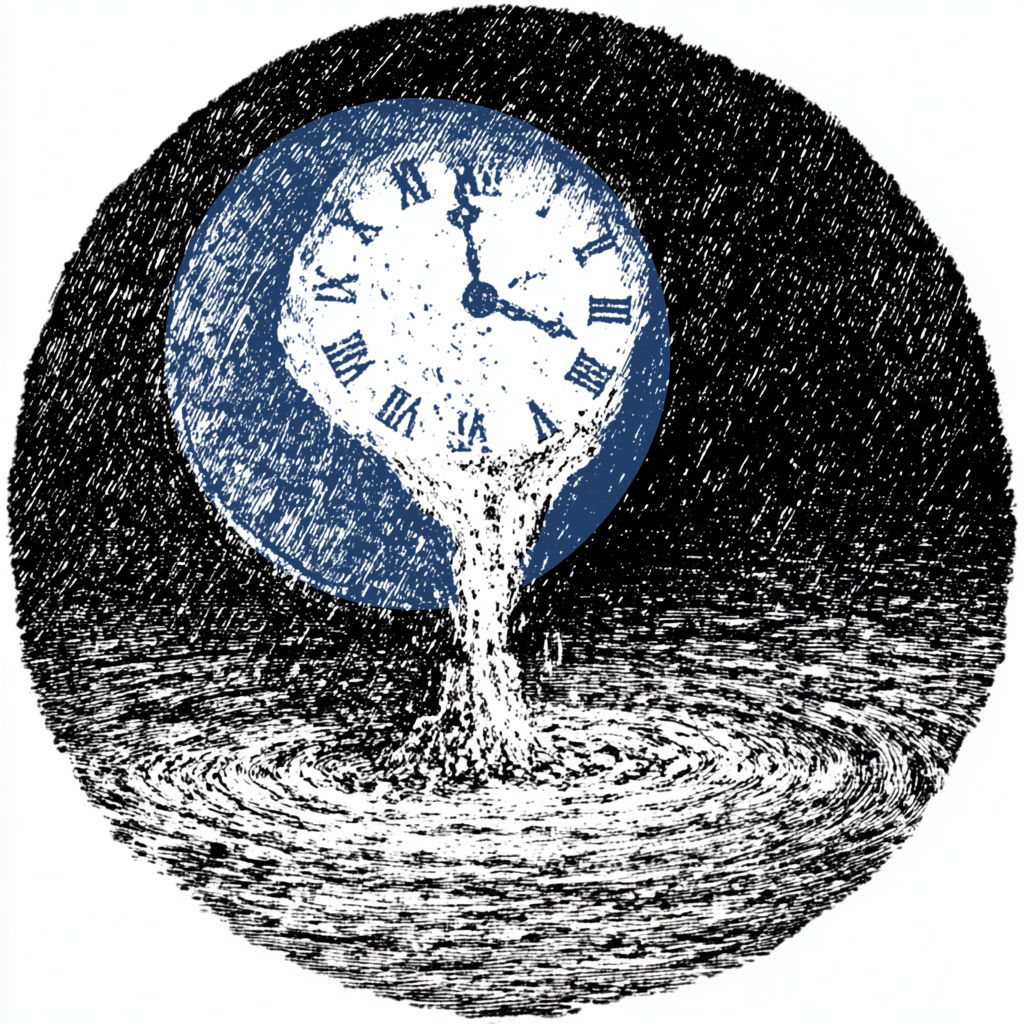
\includegraphics[width=1\linewidth]{img/clock}
  \end{center}  \vspace{-5pt}
  \emph{Time evolution gradually exchanges one state for the other.
  } \vspace{-10pt}
}
This is decreasing the amount of ``pure'' $\pi_+$ in the state by $t^2$,
filtering out $\pi_m$ from $\pi_+$ by applying the projector $\Pi_m$, and
replacing to the tune of $t^2$. In words, it appears to be
turning $\pi_+$ into $\pi_m$ at a quadratic rate in time!
Using pseudocode for Hamiltonian evolution, our algorithm is then
  \begin{minted}
     [
frame=lines,
framesep=2mm,
baselinestretch=1.2,
bgcolor=AliceBlue,
fontsize=\footnotesize,
linenos
]{slurm}
    *> def guess(t):
    ...    prop = exp(-1j*t*H)
    ...    final = prop « char(X, 0)
    ...    _, index = measure(Z, final)
    ...    return index
\end{minted}

Assuming this Hamiltonian works (you can show this is in Exercise
5.1), how quickly will it evolve $\pi_+$ to $\pi_m$?
The shortest time to evolve between states $\pi_\text{int}$ and $\pi_\text{fin}$ in a two-level system
with Hamiltonian $H$ is governed by the \emph{Rabi uncertainty relation} (Exercise 5.2)
\begin{equation}
  \label{eq:rabi}
  t^* \geq \frac{\pi}{2\sqrt{\kappa}}, \quad \kappa = [H \triangleleft \pi_\text{init}]
  \left(\Pi_\text{final}\right).
\end{equation}
We can think of $\kappa$ as a \emph{transition amplitude} between
$\pi_\text{init}$ and $\pi_\text{final}$. In our case,
\[
  \kappa = \pi_+ \left( (\Pi_m + \Pi_+)\Pi_m(\Pi_m + \Pi_+)\right) =
 4 \pi_+ \left(\Pi_m\right) = \frac{4}{d},
\]
since (by symmetry) any $Z$ projector should have the same expectation
$\pi_+ (\Pi^{(Z)}_i) = C$, and the $Z$ projectors add to unity:
\[
 1 = \pi_+ (I) =
  \sum_{i=0}^{d-1}\pi_+ (\Pi^{(Z)}_i) = dC \quad \Longrightarrow
  \quad  C = \frac{1}{d}.
\]
Thus, from (\ref{eq:rabi}), we find an optimal evolution time\sidenote{This is in agreement with the results of Farhi and
Guttman. Reference to be added.}
\begin{equation}
  \label{eq:22}
  t^* \geq \frac{\pi \sqrt{d}}{4}.
\end{equation}
Incorporating the dimension and marked item\sidenote{Strictly, we
  should replace this with dependence on the projector $\Pi_+$, but it
complicates dependencies.} as parameters, we
obtain a pseudocode search algorithm 
  \begin{minted}
     [
frame=lines,
framesep=2mm,
baselinestretch=1.2,
bgcolor=AliceBlue,
fontsize=\footnotesize,
linenos
]{slurm}
    *> def hamiltonianSearch(d, marked):
    ...    H = proj(Z, marked) + proj(X, 0)
    ...    t = pi*sqrt(d)/4
    ...    prop = exp(-1j*t*H)
    ...    final = prop « char(X, 0)
    ...    return measure(Z, final)()[1]
\end{minted}

% In order to run on a conventional \emph{digital} quantum computer, we
% need to discretize this evolution.
Evolution with this Hamiltonian is messy. We can \emph{approximate} it
using the result of Trotter and
Suzuki,\sidenote{Add reference. See Exercise 5.3.} who independently derived
\[
  e^{-it(A + B)} = \lim_{n\to\infty} \left[e^{-itA/n}e^{-itB/n}\right]^n,
\]
with an error given by\sidenote{Reference Childs et al.}
\[
  \left\Vert e^{-it(A + B)} -
    \left[e^{-itA/n}e^{-itB/n}\right]^n\right\Vert \leq \frac{t^2}{2n}
  \Vert [A, B ]\Vert.
\]
In our case, $A = \Pi_+$ and $B = \Pi_m$. The exponential simplifies
for projectors, since
\begin{align*}
  e^{-it \Pi/n} & = \sum_{k\geq 0} \frac{(-it/n)^k \Pi^k}{k!} \\ & = I +
  \Pi\sum_{k\geq 1} \frac{(-it/n)^k }{k!}  = I + (e^{-it/n} - 1) \Pi.
\end{align*}
In \texttt{yaw}, this approximation scheme becomes (real code!)
  \begin{minted}
     [
frame=lines,
framesep=2mm,
baselinestretch=1.2,
bgcolor=AliceBlue,
fontsize=\footnotesize,
linenos
]{slurm}
    *> def trotter(projList, time, steps):
    ...    factors = [I + (exp(-1j*time/steps)-1)*proj
    ...                           for proj in projList]
    ...    return prod(factors)**steps
\end{minted}
This gives a family of search algorithms, depending on the total
number of steps, or equivalently, the step size $\delta = t/n$, in
which we evolve to the final state
\begin{align}
  \pi_\text{final} & = [R_\delta(\Pi_m) R_\delta(\Pi_+)]^n
                     \triangleleft \pi_+ \\
  R_\delta(\Pi) & = e^{-i\delta \Pi} = I + (e^{-i\delta} - 1 )\Pi,
\end{align}
and measure in the $Z$ basis to make our guess $m^*$, $Z
\overset{\pi_\text{final}}{\longleftarrow} m^*$.

Continuing to assume that the algorithm
saturates the Rabi bound, we get a compact algorithm for Trotterized search:
  \begin{minted}
     [
frame=lines,
framesep=2mm,
baselinestretch=1.2,
bgcolor=AliceBlue,
fontsize=\footnotesize,
linenos
]{slurm}
    *> def trotterSearch(d, marked, time, steps):
    ...    PiList = [proj(Z, marked), proj(X, 0)]
    ...    prop = trotter(PiList, time, steps)
    ...    final = prop « char(X, 0)
    ...    return measure(Z, final)()[1]
\end{minted}
For $n$ steps and $t = \pi\sqrt{d}/4$, the error is bounded by
\[
  \frac{t^2}{2n} \Vert [\Pi_+, \Pi_-]\Vert = \frac{\pi^2d}{32n}\Vert
  [\Pi_+, \Pi_-]\Vert \leq \frac{\pi^2\sqrt{d}}{32n},
\]
where $\Vert \cdot \Vert$ indicates the largest (absolute)
eigenvalue.\sidenote{See exercises.}
% We don't really care about minimising the error; we just want our
% simulation to be good enough for \emph{search}. It is reasonable
% to accept small constant error, for instance
This means that when the number of steps $n \sim \sqrt{d}$, the error is $\mathcal{O}(1)$:
\[
  \frac{\pi^2\sqrt{d}}{32n} \sim \frac{\pi^2}{32} \approx 0.3.
  % \quad
  % \Longrightarrow \quad n = \frac{\sqrt{d}}{4}, \frac{t}{n} = \pi.
\]
Our Trotterization formula is no longer reliable here. One can show
(Exercise 5.5) that in this regime there is an additional $\pi$ in the
relation between steps and evolution time,\sidenote{This is analogous
  to the way that moving round a circle turns a
circumferential step of length $2\pi r$ into a diameter span of length $2 r$.} so that
\[
  e^{-it(A + B)} \approx \left[ R_{\pi\delta}(A) R_{\pi\delta}(B)\right]^n.
\]
and hence for $\delta = 1$ or $n = \pi\sqrt{d}/4$, we have steps
\[
  R_\pi(\Pi) = I + (e^{-i\pi} - 1) \Pi = I - 2\Pi,
\]
with $R_\pi(\Pi_m)$ the \emph{oracle reflection} and
$R_\pi(\Pi_+)$ the \emph{diffusion operator}.
Together, they give the \emph{Grover operator} $G = R_\pi(\Pi_m)
R_\pi(\Pi_+)$, with
\begin{equation}
  \label{eq:11}
\pi_\text{final} = G^n \triangleleft \pi_+, \quad Z
\overset{\pi_\text{final}}{\longleftarrow} m^*. %, G \left[ R_{\pi}(\Pi_m) R_{\pi}(\Pi_+)\right]^{\pi\sqrt{d}/4}.
\end{equation}
%Note that the discretization steps take the special form of \emph{reflections}
This is the famous discrete search algorithm of Lov Grover.\sidenote{Add references.}
\newpage
% which, physically speaking, boils down to the propagator
% \[
%   e^{-it H} \approx \left[(I - 2 \Pi_m) (I - 2 \Pi_+)\right]^{\sqrt{d}/4}.
% \]
% We can write this canonical algorithm as a special case of our
% Trotterized evolution:
%   \begin{minted}
%      [
% frame=lines,
% framesep=2mm,
% baselinestretch=1.2,
% bgcolor=AliceBlue,
% fontsize=\footnotesize,
% linenos
% ]{slurm}
%     *> def groverTrotter(d, marked):
%     ...    return search(d, marked, sqrt(d)/4)
% \end{minted}

% Although this connection between Hamiltonian search and Grover goes
% back to 1996, textbook versions of the algorithm often elide
% it.\sidenote{To be fair, Nielsen and Chuang have a good (if
%   computationally dense) discussion.} For completeness, here is
%   something closer to textbooks:
We can implement a Hamiltonian version of this algorithm, accounting
for the additional factor of $\pi$:
  \begin{minted}
     [
frame=lines,
framesep=2mm,
baselinestretch=1.2,
bgcolor=AliceBlue,
fontsize=\footnotesize,
linenos
]{slurm}
    *> def groverTrotter(d, marked):
    ...    steps, time = int(pi*sqrt(d)/4) + 1, pi*steps
    ...    return search(d, marked, time, steps)
\end{minted}
or the textbook version (with some minor refinments) as follows:
  \begin{minted}
     [
frame=lines,
framesep=2mm,
baselinestretch=1.2,
bgcolor=AliceBlue,
fontsize=\footnotesize,
linenos
]{slurm}
    *> def grover(d, marked):
    ...    $alg = qudit(d)
    ...    def reflect(P): return I - 2*P
    ...    G = reflect(proj(Z, marked)) * (-reflect(proj(X, 0)))
    ...    r = int((pi/4)*sqrt(d)) + 1  # take the ceiling
    ...    return measure(Z, (G**r) « char(X, 0))()[1]
\end{minted}
There is a minus sign in the operator $G = -R_\pi(\Pi_m)
R_\pi(\Pi_+)$, irrelevant to the final measurement, and we use the ceiling $n = \lceil
\pi\sqrt{d}/4\rceil$ for the number of steps.
Let's check that this is accurate:
  \begin{minted}
     [
frame=lines,
framesep=2mm,
baselinestretch=1.2,
bgcolor=AliceBlue,
fontsize=\footnotesize,
linenos
]{slurm}
    *> d, marked, N = 5, 3, 100
    *> sum(grover(d, marked) == marked for _ in range(N))/N
    0.96
\end{minted}
You can play around with this and see that the hit rate improves with the size
of the database!

What is the significance of this algorithm? Unlike teleportation,
which involves a new way of transmitting information, quantum
search is a new way of performing a classical task. For $d$ marked items,
Grover or Trotterized Hamiltonian evolution take $\mathcal{O}(\sqrt{d})$ steps\sidenote{In fact
  $\Theta(\sqrt{d})$ steps. Rabi establishes a lower bound, and
  the exercises show the upper bound.} to find the marked needle in the
unstructured haystack, while the best a classical computer can do is
$\mathcal{O}(d)$, since it must test every possibility until it finds
the right one.
This represents a \emph{quadratic speedup} for search, and is
a prime example of what is called \emph{quantum computational
  advantage}.
We will see a much more impressive example in a moment.